\documentclass[cjk,dvipdfmx,10pt,compress,fragile%
hyperref={bookmarks=true,bookmarksnumbered=true,bookmarksopen=false,%
colorlinks=false,%
pdftitle={第 134 回 関西 Debian 勉強会},%
pdfauthor={小林},%
%pdfinstitute={関西 Debian 勉強会},%
pdfsubject={資料},%
}]{beamer}

\title{Rustで書いたツールのdebianパッケージングに\\挑戦してみた話(仮)}
\author[Katsuki Kobayashi]{{\large\bf Katsuki Kobayashi}}
\institute[Debian JP]{{\normalsize\tt 関西 Debian 勉強会}}
\date{{\small 2019年 3月 24日 (日)}}

\usepackage{graphicx}
\usepackage{moreverb}
\usepackage{ulem}
\usepackage[varg]{txfonts}
\usepackage{tabularx}
\usepackage{fancybox}
\usepackage{fancyvrb}
\usepackage{float}
\usepackage{multicol}
\usepackage{minijs}
\usepackage{amsmath}
\usepackage{amssymb}
\usepackage{newtxtext}
\usepackage{listings, listings-rust}
\usepackage{hyperref}
\AtBeginDvi{\special{pdf:tounicode EUC-UCS2}}
\usetheme{KansaiDebian}
\def\museincludegraphics{%
  \begingroup
  \catcode`\|=0
  \catcode`\\=12
  \catcode`\#=12
  \includegraphics[width=0.9\textwidth]}
%\renewcommand{\familydefault}{\sfdefault}
%\renewcommand{\kanjifamilydefault}{\sfdefault}
%
\newenvironment{commandline}%
{\VerbatimEnvironment
  \begin{Sbox}\begin{minipage}{0.9\hsize}\begin{fontsize}{8}{8} \color{white} \begin{BVerbatim}}%
{\end{BVerbatim}\end{fontsize}\end{minipage}\end{Sbox}
  \setlength{\fboxsep}{8pt}
% start on a new paragraph

\vspace{6pt}% skip before
\fcolorbox{white}{black}{\TheSbox}

\vspace{3pt}% skip after
}
%end of commandline

\begin{document}

\begin{frame}[fragile]
\titlepage
\end{frame}

\begin{frame}[t,fragile]{自己紹介}
 \begin{itemize}
  \item Katsuki Kobayashi
	\begin{itemize}
	 \item 組み込みエンジニア
	 \item 使用言語: C, アセンブラ(ARM)
	 \item \sout{永遠}に勉強中: Python, Kotlin, アセンブラ(RISC-V), Rust
	       \onslide<2>{\item 最近会社でC++を勉強させられている。タスケテ。}
	\end{itemize}
  \item Debianとのつきあい
	\begin{itemize}
	 \item 大学時代に素敵な先輩がた(うち現在DD2名,DM1名)によって布教
	 \item 個人的にはパッケージの構成の統一感が一番好き
	 \onslide<2>{\item \sout{あんまり貢献していない}}
	\end{itemize}
  \item Rust
	\begin{itemize}
	 \item 新しい言語が勉強したい
	 \item でもPythonやRubyはネイティブなバイナリにならなくてツラい
	 \onslide<2>{\item Goが流行ってるらしい}
	 \item じゃあMozilla好きだしRustにしよう \onslide<2>{←?}
	\end{itemize}
 \end{itemize}
\end{frame}

\begin{frame}[t,fragile]{本日の流れ}
\begin{itemize}
 \item Rustをさわってみる
       \begin{itemize}
	\item rustupでツールチェーンをインストール
	\item Cargoでビルドしてみる
       \end{itemize}
 \item Rustの特徴のご紹介
       \begin{itemize}
	\item 注意: 発表者も素人なので難しい質問は回答できません
	\item \url{https://doc.rust-lang.org/stable/book/} を読んでください!!
       \end{itemize}
 \item Debianパッケージングを試してみた話
\end{itemize}
\end{frame}

\begin{frame}[t,fragile]{Rustとは?}
 \begin{itemize}
  \item Mozillaが開発したシステムプログラミング言語
	\begin{itemize}
	 \item Servo(絶賛開発中)というブラウザエンジンのために開発
	 \item 安全性・並行性について考えられて設計されている
	 \item 静的型付け言語
	\end{itemize}
  \item カニ?
	\begin{itemize}
	 \item Rustプログラマーの事をRustacean(ラストシアン)と呼ぶ
	 \item ``Crustacean(甲殻類)`` から来ているらしい
	       \begin{itemize}
		\item オライリー本の表紙はオオヒロバオウギガニ
		\item 非公式なマスコットもカニ \href{http://rustacean.net/}{(Ferrisっていう模様)}
	       \end{itemize}
	\end{itemize}
 \end{itemize}
\end{frame}

\begin{frame}[t,fragile]{インストール}
 \begin{itemize}
  \item \texttt{rustup}を入れるのが一応公式
	\begin{itemize}
	 \item \verb@curl https://sh.rustup.rs -sSf | sh@
	 \item あなたのhome dirに色々と入ります \verb@~/.cargo@
	\end{itemize}
  \item \texttt{rustup}のサブコマンドたち
	\begin{description}
	 \item[default] デフォルトのツールチェーンを切り替えます。
		    \begin{itemize}
		     \item ツールチェーン: stableかnightlyか特定のバージョンを指定できる
		    \end{itemize}
	 \item[update] 更新をかけます。
		    nightlyを使う場合はちょくちょく使う
		    \begin{itemize}
		     \item そしてたまに壊れる
		     \item 壊れるといっても、コンパイラがおかしくなった事はないです
		    \end{itemize}
	 \item[completions] シェルの補完用のコードを吐く (bash, zsh, fish, \textbf{PowerShell}, etc..)
	\end{description}
 \end{itemize}
\end{frame}

\begin{frame}[t,fragile]{Debianパッケージでのインストール}
 \begin{itemize}
  \item もちろんDebianのパッケージもある
	\begin{itemize}
	 \item ビルドツールであるcargoのパッケージを入れるのがよろしいかと
	 \item 一緒にコンパイラ(rustc)も入ります
	\end{itemize}
 \end{itemize}
 \begin{commandline}
% apt show cargo
Package: cargo
Version: 0.33.0-1
Priority: optional
Section: rust
Maintainer: Rust Maintainers <pkg-rust-maintainers@alioth-lists.debian.net>
Installed-Size: 9,453 kB
Depends: libc6 (>= 2.18), libcurl3-gnutls (>= 7.28.0), libgcc1 (>= 1:4.2), \
libgit2-27 (>= 0.26.0), libssh2-1 (>= 1.2.5), libssl1.1 (>= 1.1.0), \
zlib1g (>= 1:1.1.4), rustc (>= 1.24), binutils, gcc | clang | c-compiler
Suggests: cargo-doc, python3
Homepage: https://crates.io/
Download-Size: 2,483 kB
APT-Manual-Installed: yes
APT-Sources: http://ftp.jp.debian.org/debian sid/main amd64 Packages
 \end{commandline}
\end{frame}

\begin{frame}[t,fragile]{Hello World (1/4)}
 \begin{itemize}
  \item Rustのプロジェクトは、 \verb|cargo new| で作ります
	\begin{itemize}
	 \item \verb|--bin| (現default) か \verb|--lib| (旧default) でパッケージの種類も指定できます
	\end{itemize}
 \end{itemize}
\begin{commandline}
% cargo new hello
     Created binary (application) `hello` package
\end{commandline}
\begin{itemize}
 \item 実行すると、Cargo.tomlとsrc/main.rsができる
\end{itemize}
\begin{commandline}
% tree
.
├── Cargo.toml
└── src
    └── main.rs

1 directory, 2 files
\end{commandline}
\end{frame}

\begin{frame}[t,fragile]{Hello World (2/4)}
 \begin{itemize}
  \item 実はプロジェクトを作った時点でHello Worldの半分が完了している
	\begin{itemize}
	 \item 生成されたsrc/main.rsの中身↓
	\end{itemize}
 \end{itemize}
\begin{lstlisting}[language=Rust,style=boxed,style=colouredRust]
fn main() {
    println!("Hello, world!");
}\end{lstlisting}
\begin{itemize}
 \item 実行するには \verb|cargo run|
\end{itemize}
\begin{commandline}
% cargo run
   Compiling hello v0.1.0 (/path/to/hello)
    Finished dev [unoptimized + debuginfo] target(s) in 0.31s
     Running `target/debug/hello`
Hello, world!
\end{commandline}
\end{frame}

\begin{frame}[t,fragile]{Hello World (3/4)}
\begin{itemize}
 \item 少しコードを見てみる
\end{itemize}
\begin{lstlisting}[language=Rust,style=boxed,style=colouredRust]
fn main() {
    println!("Hello, world!");
}\end{lstlisting}
 \begin{description}
  \item[関数定義] \verb|fn|を使う
  \item[main関数] 戻り値は書かない
  \item[\texttt{println!()}] 実は関数ではなくてマクロ (\verb|!|が付いてるのはマクロ)
 \end{description}
\end{frame}

\begin{frame}[t,fragile]{Hello World (4/4)}
\begin{itemize}
 \item Cargo.toml
\end{itemize}

\begin{commandline}
[package]
name = "hello"
version = "0.1.0"
authors = ["Katsuki Kobayashi <katsuki.kobayashi@gmail.com>"]
edition = "2018"

[dependencies]
\end{commandline}

\begin{itemize}
 \item Cargo.lock (ビルドすると自動生成)
\end{itemize}

\begin{commandline}
# This file is automatically @generated by Cargo.
# It is not intended for manual editing.
[[package]]
name = "hello"
version = "0.1.0"
\end{commandline}
\end{frame}

\begin{frame}[t,fragile]{それじゃあ……}
\begin{itemize}
 \item ちょっと色々とRustの構文とか機能を紹介します
       \begin{itemize}
	\item 解らない or もっと詳しくと思ったらThe bookを読んでもらえればと
	      \begin{itemize}
	       \item 口頭で聞いてもらっても良いですが回答に窮する可能性が高いです \verb|;-)|
	      \end{itemize}
	\item The book: \url{https://doc.rust-lang.org/stable/book/}
	\item 実行環境はwebでやってもらっても良いかもです
	      \begin{itemize}
	       \item \url{https://play.integer32.com/}
	      \end{itemize}
       \end{itemize}
 \item まじめに向き合うには結構大変
       \begin{itemize}
	\item カニ本で引用されてる
	      \href{https://www.quora.com/What-do-C-C++-systems-programmers-think-of-Rust/answer/Mitchell-Nordine}{Quoraの記事}
	\item C++の本を現在進行形で読んでる身にはすごく納得
	      \begin{itemize}
	       \item 大体、C++11ではこう書けるからそれが推奨っていうのがRustの文法
	      \end{itemize}
       \end{itemize}
\end{itemize}
\begin{quote}
I've found that Rust has forced me to learn many of the things that I was slowly learning as "good practise" in C/C++ before I could even compile my code.
\end{quote}
\end{frame}

\begin{frame}[t,fragile]{変数宣言(1/3)}
\begin{lstlisting}[language=Rust,style=boxed,style=colouredRust]
    let x = 1;
    println!("x = {}", x);
    let x = 1.25;
    println!("x = {}", x);
    // x = 1;   // error: expected floating-point number,
                // found integer
    // x = 1.5; // error: cannot assign twice to
                // immutable variable\end{lstlisting}
\begin{itemize}
 \item 変数の宣言はletで行なう
       \begin{itemize}
	\item 型は(一意に推論できるなら)省略可能
	\item シャドーイング可能
	\item 指定がなければimmutableな変数になる
       \end{itemize}
\end{itemize}
\end{frame}

\begin{frame}[t,fragile]{変数宣言(2/3)}
\vspace*{-2zw}
\begin{lstlisting}[language=Rust,style=boxed,style=colouredRust]
    let mut y: u32 = 1;
    y -= 1;
    y -= 1;
    println!("y = {}", y);\end{lstlisting}
\begin{itemize}
 \item 変数の宣言はletで行なう
       \begin{itemize}
	\item 型は後置貴方(コロンの後ろにつける)
	\item mutableな変数にしたければ \texttt{mut} キーワードを使う
       \end{itemize}
 \item ちなみに、実行するとデバッグビルドだと途中で止まります
\end{itemize}
\begin{commandline}
% cargo run
Compiling variable v0.1.0 (/path/to/examples/variable)
Finished dev [unoptimized + debuginfo] target(s) in 0.00s
Running `target/debug/variable`
thread 'main' panicked at 'attempt to subtract with overflow', \
variable/src/main.rs:12:5
note: Run with `RUST_BACKTRACE=1` environment variable to \
display a backtrace.
\end{commandline}
\end{frame}

\begin{frame}[t,fragile]{変数宣言(3/3)}
 \begin{itemize}
  \item リリースビルド(\verb|--release|付き)すると最後まで実行する
	\begin{itemize}
	 \item もちろん、結果はおかしなことになる
	\end{itemize}
 \end{itemize}
\begin{commandline}
% cargo run
Compiling variable v0.1.0 (/path/to/examples/variable)
Finished release [optimized] target(s) in 0.30s
Running `target/release/variable`
x = 1
x = 1.25
y = 4294967295
\end{commandline}
\end{frame}

\begin{frame}[t,fragile]{基本的な型}
 \begin{description}
  \item[整数]
	      \textbf{符号無し:} \texttt{u8}, \texttt{u16}, \texttt{u32}, \texttt{u64}, \texttt{usize}\\
	      \textbf{符号付き:} \texttt{i8}, \texttt{i16}, \texttt{i32}, \texttt{i64}, \texttt{isize}
  \item[浮動小数点] \textbf{単精度:} \texttt{f32}、\textbf{倍精度:} \texttt{f64}
  \item[ブール] \texttt{bool}
  \item[文字] \texttt{char}  (Unicodeの1文字)
  \item[文字列] \texttt{String}
	     \begin{itemize}
	      \item ただし、文字列リテラルの \texttt{str} があってとてもややこしい
	     \end{itemize}
  \item[配列] \texttt{[T; N]} (\texttt{T}: 型,  \texttt{N}: 要素数)
  \item[ベクター] \texttt{Vec<T>} (\texttt{T}: 型)
  \item[スライス] \texttt{\&[T]} (\texttt{T}: 型)
 \end{description}
\end{frame}

\begin{frame}[t,fragile]{\texttt{String}と\texttt{str} (1/2)}
\begin{itemize}
 \item C++の\texttt{std::string}と\texttt{char}に似ている
\end{itemize}
\begin{lstlisting}[language=Rust,style=boxed,style=colouredRust]
    let a = "abcd".to_string(); // String::from("abcd"); も可
    let b = &a[1..];
    let c = "zyxwv";\end{lstlisting}
\begin{center}
 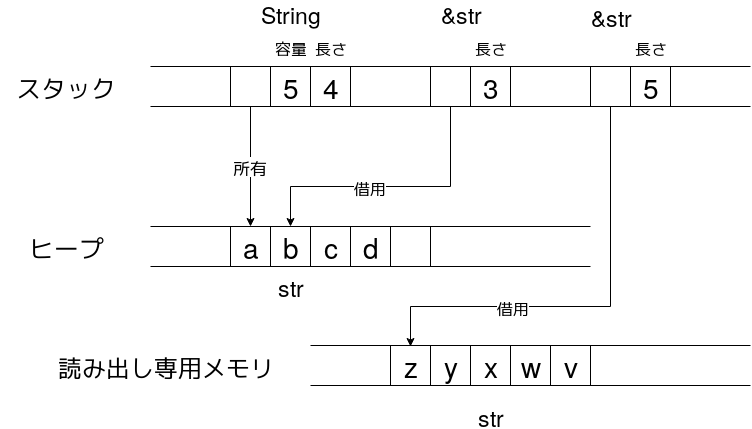
\includegraphics[keepaspectratio,height=4cm]{./img/rustlang-str-string.png}
\end{center}
\end{frame}

\begin{frame}[t,fragile]{\texttt{String}と\texttt{str} (2/2)}
\begin{itemize}
 \item \texttt{String}は可変長
\end{itemize}
\begin{lstlisting}[language=Rust,style=boxed,style=colouredRust]
    let mut a = "abcd".to_string();
    //  ^^^
    a.push_str("efg");  // OK

    let mut c = "zyxwv";
    // no method named `push_str` found
    // for type `&str` in the current scope
    c.push_str("ut");  // Error!! \end{lstlisting}
\end{frame}

\begin{frame}[t,fragile]{関数}
 \begin{itemize}
  \item \texttt{fn} キーワードと \texttt{->} トークンを使って書く
 \end{itemize}
\begin{lstlisting}[language=Rust,style=boxed,style=colouredRust]
fn add(a: i32, b: i32) -> i32 {
    return a + b;
}

fn main() {
    println!("{}", add(1, 2));
}\end{lstlisting}

\begin{commandline}
% cargo run
Compiling function v0.1.0 (/path/to/examples/function)
Finished dev [unoptimized + debuginfo] target(s) in 0.20s
Running `target/debug/function`
3
\end{commandline}
\end{frame}

\begin{frame}[t,fragile]{所有権(1/4)}
 \begin{itemize}
  \item 整数型と文字列型の変数を複数の変数に代入してみる
	\begin{itemize}
	 \onslide<2>{\item どうなると思います?}
	\end{itemize}
 \end{itemize}
 \begin{lstlisting}[language=Rust,style=boxed,style=colouredRust]
    let i0 = 1;
    let i1 = i0;
    let i2 = i0;

    let s0: String = "hoge".to_string();
    let s1 = s0;
    let s2 = s0;\end{lstlisting}
\end{frame}

\begin{frame}[t,fragile]{所有権(2/4)}
\begin{itemize}
 \item 文字列型の方だけコンパイルエラーになる
       \begin{itemize}
	\item Rustでは、代入、関数の引数、関数の戻り値で
	      所有権が移動する
	\item ただし、整数等、一部の型はコピーになる
	      \begin{itemize}
	       \item そのため\verb|i2|ではエラーになっていない
	       \item コピーされる型については、
		     エラーで出ている ``Copy trait '' というのがミソ
	      \end{itemize}
       \end{itemize}
\end{itemize}
\begin{commandline}
error[E0382]: use of moved value: `s0`
 --> ownership/src/main.rs:8:15
  |
6 |     let s0: String = "hoge".to_string();
  |         -- move occurs because `s0` has type `std::string::String`, \
               which does not implement the `Copy` trait
7 |     let s1 = s0;
  |              -- value moved here
8 |     let s2 = s0;
  |              ^^ value used here after move
\end{commandline}
\end{frame}

\begin{frame}[t,fragile]{所有権(3/4)}
\begin{itemize}
 \item 関数の引数も駄目なので以下もアウト
\end{itemize}
 \begin{lstlisting}[language=Rust,style=boxed,style=colouredRust]
fn consume(_s: String) {}
// 中略
    let h: String = "Hello World".to_string();
    consume(h);
    let hh = h;
\end{lstlisting}

\begin{commandline}
12 |     let h: String = "Hello World".to_string();
   |         - move occurs because `h` has type `std::string::String`, \
               which does not implement the `Copy` trait
13 |     consume(h);
|                - value moved here
14 |     let hh = h;
|                 ^ value used here after move
\end{commandline}
\end{frame}

\begin{frame}[t,fragile]{所有権(4/4)}
\begin{itemize}
 \item 逆に関数の戻り値の所有権を呼び元に渡せる
\end{itemize}
 \begin{lstlisting}[language=Rust,style=boxed,style=colouredRust]
fn generate(i: i32) -> Vec<i32> {
    let mut v = Vec::new();
    v.push(i);
    return v;
}
// 略
    let v1 = generate(10);
    let mut v2 = generate(100);
    v2.push(101);
    println!("v1: {:?}", v1); // v1: [10]
    println!("v2: {:?}", v2); // v2: [100, 101]\end{lstlisting}
\end{frame}

\begin{frame}[t,fragile]{参照, 借用}
 \begin{itemize}
  \item 所有権を渡したい場合には参照を使う
	\begin{itemize}
	 \item Rustでは「借用」とも言う
	\end{itemize}
 \end{itemize}
\end{frame}

\takahashi[30]{ようやくDebian要素}

\begin{frame}[t,fragile]{Debianパッケージにしてみる}
 \begin{itemize}
  \item 一番簡単な方法 : \texttt{cargo-deb}
	\begin{itemize}
	 \item A cargo subcommand that generates Debian packages from information in Cargo.toml
	       \begin{itemize}
		\item \href{https://github.com/mmstick/cargo-deb}{GitHub}
		\item \href{https://users.rust-lang.org/t/cargo-deb-make-debian-packages-from-cargo-projects/12199}{アナウンス@users.rustlang.org}
	       \end{itemize}
	 \item インストール方法
	       \begin{itemize}
		\item \verb|cargo install cargo-deb|
		\item debは……ない……!!
	       \end{itemize}
	 \item 問題点
	       \begin{itemize}
		\item 公式にはとても入らないdebを吐く
		\item 単一バイナリのプロジェクトにしか対応していない
	       \end{itemize}
	 \item まぁ、えいやと/usr/binに入れたいならアリかもですが……
	\end{itemize}
 \end{itemize}
\end{frame}

%\begin{frame}[t,fragile]{真面目にDebianパッケージにしてみる}
% 
%\end{frame}

\begin{frame}[t,fragile]{\texttt{dh\_make}する}
\begin{commandline}
% dh_make -p rwget_0.1.0 --createorig
Type of package: (single, indep, library, python)
[s/i/l/p]?
Maintainer Name     : Katsuki Kobayashi
Email-Address       : rare@tirasweel.org
Date                : Sun, 17 Mar 2019 20:33:47 +0900
Package Name        : rwget
Version             : 0.1.0
License             : blank
Package Type        : single
Are the details correct? [Y/n/q]
Currently there is not top level Makefile. This may require additional tuning
Done. Please edit the files in the debian/ subdirectory now.
\end{commandline}
\end{frame}

\takahashi[50]{以上}

\begin{frame}[t,fragile]{どっかに挿入予定のメモ}
 \begin{itemize}
  \item Rustのファイルの拡張子は .rs
	\begin{itemize}
	 \item Rustで書かれたプロジェクトの公式サイトが \verb|http://xxx.rs| であることが多い
	 \item 国別コードトップドメイン .rs : セルビア
	\end{itemize}
  \item \texttt{rust-fmt}というツールがある
	\begin{itemize}
	 \item \texttt{gofmt}とか\texttt{autopep8}とか\texttt{clang-format}的なツール
	\end{itemize}
  \item Podcast (Rebuild.fm?) で誰かが言ってた
	\begin{itemize}
	 \item Go: C++が嫌いで駆逐したい
	 \item Rust: C++が大好きだけど辛いのでなんとかしたい
	\end{itemize}
  \item Rustacean
	\begin{itemize}
	 \item LISPer, Pythonista, Rubyist, Gopher, TeXnician的な
	 \item ``crustaceans'' : 甲殻類
	       \begin{itemize}
		\item オライリー本の表紙はオオヒロバオウギガニ
		\item 非公式なマスコットもカニ \href{http://rustacean.net/}{(Ferrisっていう模様)}
	       \end{itemize}
	\end{itemize}
 \end{itemize}
\end{frame}

\begin{frame}[t,fragile]{どっかに挿入予定のメモ}
 \begin{itemize}
  \item とりあえずパッケージにするには
	\begin{itemize}
	 \item \verb|dh_make| を実行
	 \item debian/rulesの\texttt{dh}の引数に\verb|--buildsystem cargo|を追加
	\end{itemize}
 \end{itemize}
 \begin{commandline}
cp: './debian/cargo-checksum.json' を stat できません: \
そのようなファイルやディレクトリはありません
 \end{commandline}
 \begin{itemize}
  \item むぅ?
	\begin{itemize}
	 \item \texttt{cargo-vendor}で各crateのchecksumは作れるけど、
	       \texttt{main.rs}なアプリはどうしたら?
	\end{itemize}
 \end{itemize}
\end{frame}

\begin{frame}[t,fragile]{どっかに挿入予定のメモ}
\begin{commandline}
debian cargo wrapper: running subprocess (['env', 'RUST_BACKTRACE=1', '/usr/bin/cargo', '-Zavoid-dev-deps', 'build', '--verbose', '--verbose', '-j4', '--target', 'x86_64-unknown-linux-gnu'],) {}
error: no matching package named `hyper` found
\end{commandline}
\end{frame}

\begin{frame}[t,fragile]{どっかに挿入予定のメモ}
 \begin{itemize}
  \item \texttt{debcargo}, \texttt{debcargo-conf}
	\begin{itemize}
	 \item crate.ioに存在するcrateにしか対応していない模様
	\end{itemize}
 \end{itemize}
\end{frame}

\end{document}